\documentclass[
  accentcolor=tud1c,	% Color theme for TUD corporate design
  colorbacktitle,		% Titlepage has colored background for title area
  inverttitle,			% Font color of title on titlepage is inverted
  german,
  twoside
]{tudreport}

% usepackages
\usepackage[ngerman]{babel}
\usepackage[utf8]{inputenc}
\usepackage{graphicx}
\usepackage{listings}
\usepackage{hyperref}

% define C++ listings style
\definecolor{commentgreen}{RGB}{50,127,50}
\lstloadlanguages{C++,[gnu]make}
\lstset{language=C++}
\lstset{captionpos=b}
\lstset{tabsize=3}
\lstset{breaklines=true}
\lstset{basicstyle=\ttfamily}
\lstset{columns=flexible,keywordstyle=\color{purple},stringstyle=\color{blue},commentstyle=\color{commentgreen}}
\lstset{literate=%
	{Ö}{{\"O}}1
	{Ä}{{\"A}}1
	{Ü}{{\"U}}1
	{ß}{{\ss}}2
	{ü}{{\"u}}1
	{ä}{{\"a}}1
	{ö}{{\"o}}1
	{'}{{\textquotesingle}}1
}

% intendation depth of parentheses
\parindent0pt

\title{Cheatsheet zum\linebreak[1]C/C++-Praktikum\linebreak[1] Fachgebiet Echtzeitsysteme}

\begin{document}

\maketitle

\chapter{Eclipse Tutorial}

\section{Neues Projekt anlegen}
Um ein neues Projekt anzulegen, wähle \textbf{File $\rightarrow$ New $\rightarrow$ C++ Project} im Eclipse Menü.
Gib den gewünschten Projektnamen ein und wähle \textbf{Empty Project} als Projekttyp aus.

\section{Neue Dateien zum Projekt hinzufügen}
Um eine neue Sourcecode-Datei zum Projekt hinzuzufügen, klicke mit der rechten Maustaste auf das Projekt und wähle \textbf{New $\rightarrow$ Source File}.
Gib einen Dateinamen (z.B. \texttt{main.cpp}) ein und bestätige mit \textbf{Finish}.
Verfahre analog, um Header-Dateien zu erstellen, wähle jedoch \textbf{New $\rightarrow$ Header File} im Kontextmenü.
Sourcecode-Dateien tragen in der Regel die Endung \emph{.cpp}, Header-Dateien \emph{.h} oder \emph{.hpp}.

\subsection{Neue Klassen zum Projekt hinzufügen}
Für eine Klasse kann man Header- und Sourcecode-Datei in einem Schritt erzeugen.
Wähle dazu \textbf{New $\rightarrow$ Class} im Kontext-Menü des Projekts, um den entsprechenden Wizard zu starten.
Gib den Namen und bei Bedarf den Namespace sowie weitere Informationen wie z.B. die Elternklassen ein (dazu später mehr).
Setze für die ersten Aufgaben den \textbf{virtual} Modifier des Destruktors auf \textbf{No}.


\section{Projekt kompilieren und starten}
Bevor ein C++-Programm gestartet werden kann, muss es kompiliert werden.
Im Gegensatz zu Java wird der Compiler nicht automatisch von Eclipse im Hintergrund aufgerufen, sondern muss manuell gestartet werden.
Um das aktuell offene Projekt zu kompilieren, klicke auf das \textbf{Build-}Symbol (\glqq Hammer\grqq) in der Eclipse C++ Toolbar.
Im \textbf{Console-}Fenster unten werden Compiler-Meldungen und eventuelle Fehler während des Erstellungsprozesses angezeigt.

Öffne zum Starten des Programms das Kontextmenü des Projekts und wähle \textbf{Run As$\rightarrow$ Local C/C++ Application }.
Danach kannst du zum Starten den grünen Run-Knopf benutzen.

\subsection{Projekt debuggen}
Du kannst dein Programm auch im Debug-Modus laufen lassen, um dir Schritt für Schritt den Ablauf anzusehen und mögliche Fehler zu finden.
Zum Debuggen wählst du (wie auch bei Java) den Debug-Knopf (\glqq Käfer\grqq) und Eclipse wird automatisch in die Debug-Perspektive wechseln.

\chapter{C++}
%C++:
% - Pointer, Referenzen, Doppelpointer
% - nützliche Header
% - 0, NULL <- cstddef.h
% - Schleifenkonstrukte
%   * reguläre for loop
%   * iterator-basierte for loop
%   * while-do, do-while
% - try-catch
% - Generisches Klassentemplate?
% - Syntax für Funktionspointer. Wie liest man den Typ eines Funktionspointers.
%
%C++11 (merge mit C++):
% - "nullptr"
% - foreach	(3 for schleifen varianten zeigen: normal, iterator, foreach)
% - shared_ptr
% - lambdas?
%

\chapter{Mikrocontroller}

\begin{center}
	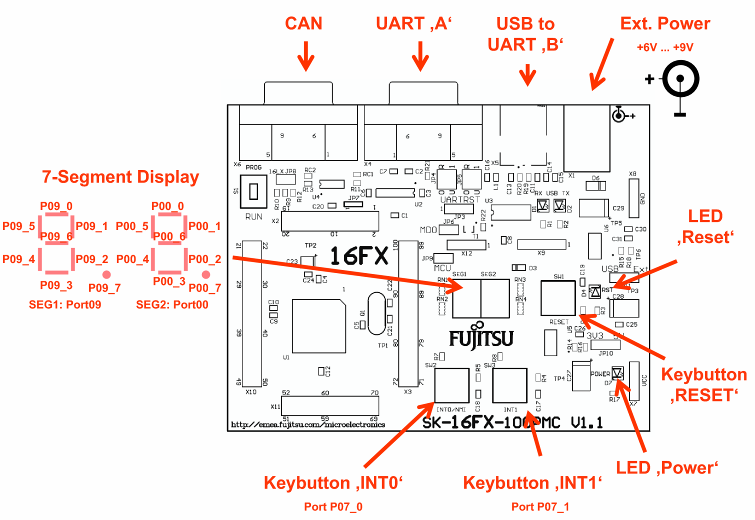
\includegraphics[width=0.6\textwidth]{figures/starterkit.png}
\end{center}


\section{C}
\subsection{Minimalprogramm}
Folgendes Programm läuft bleibt unendlich lange in der for-Schleife und führt bei jedem Durchgang eine Warteoperation durch.
Die Include-Anweisung ist notwendig, um das Programm auf dem Mikrocontroller zu verwenden.
Es bietet Zugang zur Hardware, als auch Systemfunktionen wie zum Beispiel die Warteoperation.
% TODO wozu NOP?
\begin{lstlisting}
#include "mb96348hs.h"
void main(void) {
	for (;;) {
		__wait_nop();
	}
}
\end{lstlisting}
% - generisches Programm: main loop, Variablen müssen am Anfang des Scopes deklariert werden
% - Ansteuerung 7-Segment-Anzeige
% - Auslesen Taster
% - Auslesen Poti
% - Ansteuerung LCD

\end{document}
